\documentclass[12pt]{article} %,fleqn
\usepackage{Diplo}

\usepackage[left=3cm,right=1.5cm,
top=2cm,bottom=2cm]{geometry}

\usepackage{comment}
\usepackage{hyperref}
\newtheorem{definition}{Определение}
\newtheorem{theorem}{Теорема}
\newtheorem{utv}{Утверждение}

\graphicspath{{../pics/}}


\begin{document}
	
\vskip 3mm

\setcounter{page}{1}
%%%%%%%% Титульный лист %%%%%%%%%%%%%%%%%%%%%%%%%%%%%%%%%
\begin{center}
	\thispagestyle{empty}
	
	{ Министерство науки и высшего образования Российской Федерации\\}

	
	
	{ Московский Физико-технический институт \\}
	
	{ (Государственный Университет) \\}
	
	{ Факультет управления и прикладной математики  \\}
	
	{ Кафедра Интеллектуальных систем\\}
	
	{при Вычислительном Центре им. А.А.Дородницына РАН\\ [4cm]}
	
	{ \bf \Large Выпускная квалификационная работа\\}
	
	{ \bf \Large{"Разработка метода выделения века как параметрической кривой на изображении глаза"\\[1cm]} }
	
	{\bf {Студента 4-го курса Ефремова Сергея Владимировича}\\[3cm]}
	
\end{center}

\begin{flushright}
	\bf{Научный руководитель}\\
	\bf{д-р техн. наук Матвеев И. А.}\\[4cm]
\end{flushright}


\begin{center}
	Москва, 2020
\end{center}
%%%%%%%%%%%%%%%%%%%%%%%%%%%%%%%%%%%%%%%%%%%%%%%%%%%%%%%%%%%%%%%%

\newpage
\begin{abstract}
	{}
	

\end{abstract}

\newpage
\tableofcontents
 


\newpage
\section{Введение}

Благодаря стремительному развитию технологий, с каждым днём все больше расширяется сфера практического применения технических средств цифровой обработки изображений. При этом относительно новым направлением стала разработка методов распознавания личности на основе человеческого глаза. Идентификация личности человека по радужке – перспективное направление развития, которое может быть использовано в системах контроля доступа. 

Интересно то, что эта идея не нова, так, еще в 1936 году офтальмологи \cite{Medic} предложили использовать для этих целей радужную оболочку глаза (рис.~\ref{fig:glaz}). Далее исследователями всего мира разрабатывались различные методы распознавания человека по его радужной оболочке, но по-настоящему сильный рост интереса к идентификации произошел только в начале XXI века. Это объяснялось качественными изменения условий жизнь общества: эволюция средств регистрирования и обработки изображений, необходимость распознавания личности в связи с террористической угрозой\cite{Conf3, Terr, Tech}. 

\begin{figure}[h]
	
	\centering
	
	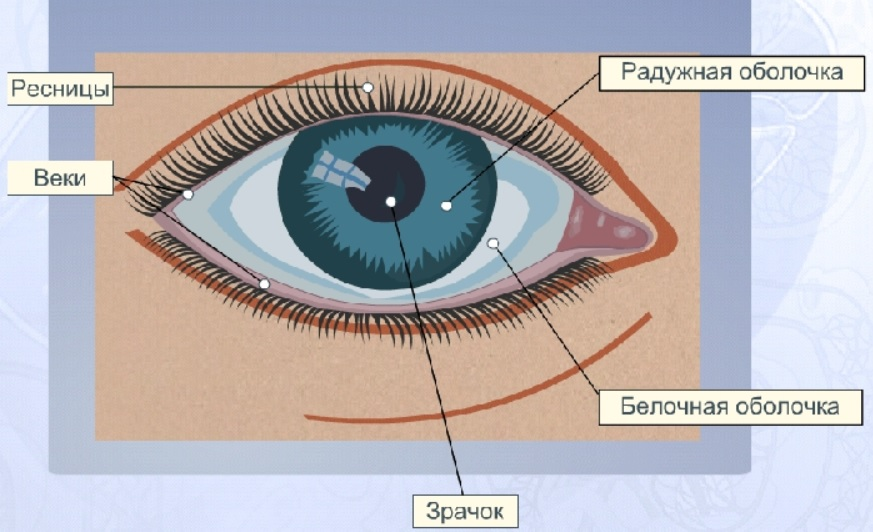
\includegraphics[width=0.6\linewidth]{glaz.jpg}
	
	\caption{Внешнее строение глаза}
	
	\label{fig:glaz}
	
\end{figure}

Однако получить качественное и обособленное изображение радужки на практике становится не так просто, и важной задачей оказывается необходимость корректно определять границы глаза, задаваемые веками. Исследования в этом направлении породили различные модели, которые также используют в биометрических системах распознавания личности. 

На сегодняшний день можно с уверенностью говорить о том, что биометрические технологии идентификации личности плотно вошли в нашу жизнь и используются во всех сферах человеческой деятельности, в том числе и в системах контроля. Так, существует целый ряд биометрических модальностей, позволяющих идентифицировать человека: рисунок папиллярных линий пальца, радужка глаза, походка, голос, почерк. Такое разнообразие методов объясняется тем, что при богатстве потенциальных сценариев использования биометрических модальностей, каждая из них может быть использована по-разному для аутентификации пользователя. Например, применение биометрических технологий уже активно осуществляется при проведении платежных операций в банковской сфере, особо нуждающейся в защите данных. Здесь они заменяют уже ставшие традиционными методы идентификации пользователей: ПИН-коды, пароли и т.д. Однако, биометрические технологии имеют широкую перспективу использования, так как обладают целым рядом неоспоримых преимуществ. Среди которых можно выделить невозможность кражи ключа без ведома его обладателя.

Использование биометрических систем настолько плотно вошло в нашу жизнь, что обыватель даже не замечает, как часто и повсеместно ими пользуется. Так, в частности, для разблокировки мобильных устройств, применяется отпечаток пальца, снимок лица или радужки. Еще одним преимуществом биометрических систем, в частности идентификации человека по его радужной оболочке, считается удобство взаимодействия с ними пользователя. Эффективность работы систем основывается на способности обработки поступающих в них данных с учетом изменчивости состояния и условий окружающей среды. То есть, даже в случае значительных искажений параметров входящих данных, в связи с изменчивостью состояний (например, ухудшение условий освещенности, затемнение ресницами, отвод взгляда), системы биометрической идентификации, использующие изображения глаза, должны выдавать корректный результат и аутентифицировать пользователя адекватно. Также неоспоримо важным фактором для эффективности систем такого рода, является необходимость работы в условиях ограниченности не только вычислительных ресурсов, но и времени, требующегося на распознание.
Однако хотелось бы отметить, что обработка изображения радужки необходима не только для идентификации человека, но и применяется в медицинских целях, что еще больше подчеркивает необходимость и важность получения корректной информации. 

\newpage
В связи со всем вышеперечисленным, в ходе данного исследования был разработан метод выделения века как параметрической кривой на изображении глаза. Представленный метод основан на том, что параметры искомой кривой определяются с помощью максимизации суммы вертикального градиента яркости, рассматриваемого в окрестности века. Стоит учитывать, что большинство, существовавших ранее методов, основывались на определении полной границы века или границы радужки целиком, но ни один из них не предлагал осуществлять обработку в несколько этапов, как в данной работе.
 

\newpage
\subsection{Цели и задачи работы}

\textbf{Цель и задачи исследования.} Основной целью исследования является построение модели, позволяющей определять коэффициенты параболы, задающей положение верхнего века и улучшить качество выделения по сравнению с существующими моделями. Для реализации этой цели были поставлены следующие задачи:
\begin{itemize}
	\item Изучить существующие подходы к решению задачи выделения века на изображении глаза.
	\item Изучить существующие алгоритмы решения этой задачи.
	\item Провести предобработку данных.
	\item Реализовать алгоритмическую часть модели, построенной на идее оптимизации и градиентного анализа.
	\item Модернизировать модель определения крайней точки века с помощью многонаправленного двумерного (2D) фильтра Габора и метода скользящего окна. 
	\item Реализовать модернизированную модель и сравнить полученные результаты с существующими алгоритмами.
\end{itemize}

\bigskip

\textbf{Научная новизна.} Используется принципиально новый подход к определению коэффициентов квадратичной параболы, задающей веко, с помощью оптимизации градиентного функционала.

\bigskip

\textbf{Методы исследования.} Алгоритмы реализованы на языке программирования C++ с использованием библиотеки OpenCV~3.4.

\bigskip

\textbf{Практическая ценность.} Полученная модель может быть использована в качестве встраиваемого модуля. Например, с её помощью можно
\begin{enumerate}
	\item Фиксировать границы зрачка глаза для последующей идентификации личности по радужке с более точным результатом.
	\item Дополнять существующие биометрические системы с помощью идентификации не только радужки испытуемого, но и линии века, получая более высокое качество распознавания.
\end{enumerate}
%%%%%%%%%%%%%%%%%%%%%%%%%%%%%%%%%%%%%%%%%%%%%%%%%%%%%


\newpage
\section{Определения и обозначения}

\subsection{Основные определения и понятия}

\textcolor{red}{Возможно блок лишний и его стоит убрать?}

\textcolor{red}{Какого рода терминологию сюда стоило бы включить?}

\subsection{Постановка задачи}
\textcolor{red}{Оставлю пока это тут.}

\textcolor{red}{
	В процессе исследования предлагается в начале определить одну точку верхнего века, а затем на основании этой точки изучать её окрестность и подбирать параметрические коэффициенты, исследуя оптимизируемый функционал. Точка, о которой идет речь обозначена на рис.~\ref{fig:glaz2} литерой $V$.
	Метод дает возможность выявить положение верхнего века после определения положения зрачка, причём с высокой точностью. В связи с тем, что он отличается высокой скоростью работы и устойчивостью, возможно его применение в широком круге систем биометрической аутентификации.}

\begin{figure}[h]
	
	\centering
	
	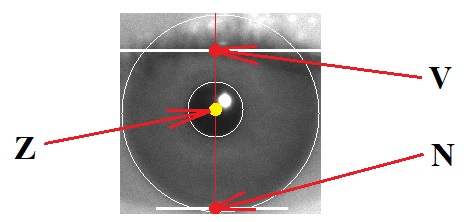
\includegraphics[width=0.6\linewidth]{glaz2.jpg}
	
	\caption{Положение век. V и N~--- точки, соответствующие положениям верхнего и нижнего век соотвественно, Z~--- центр зрачка}
	
	\label{fig:glaz2}
	
\end{figure}

%%%%%%%%%%%%%%%%%%%%%%%%%%%%%%%%%%%%%%%%%%%%%%%%%%%%%

\newpage
\section{Обзор существующих методов}

\subsection{Методы выделения контуров}

Практически все методы выделения контуров основываются на разрывности сигнала яркости. Наиболее общим способом поиска перепадов яркостей является обработка изображения методом скользящего окна, называемого в разной литературе также маской, фильтром, ядром или шаблоном. Оно представляет из себя некую прямоугольную матрицу, накладываемую на группу пикселей исходного изображения. Элементы такой матрицы называют коэффициентами, а разного рода преобразования над ней~--- фильтрацией или пространственной фильтрацией(рис.~\ref{fig:prost_filt}).

\begin{figure}[h]
	
	\centering
	
	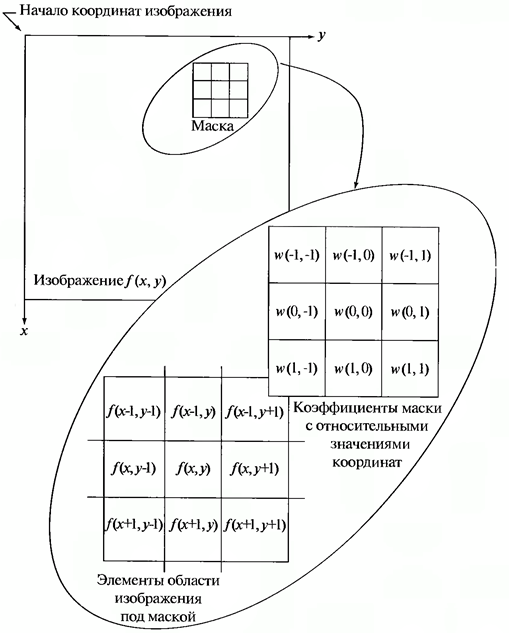
\includegraphics[width=0.7\linewidth]{prost_filt.jpg}
	
	\caption{Схема пространственной фильтрации}
	
	\label{fig:prost_filt}
	
\end{figure}

\newpage

Процесс основан на перемещении фильтра от точки к точке, вычисляя отклик для каждой из них. Для случая линейной пространственной фильтрации значение задается суммой произведения коэффициентов маски на соотвествующие значения яркостей в точках, покрытых маской. Так, для квадратной маски размерности $3\times3$ отклик $R$ линейной фильтрации в точке $(x, y)$ изображения на рис.~\ref{fig:prost_filt} определится как сумма произведений значений маски на значнения пикселей под маской:
\begin{gather}\label{3.1}
R = w(-1,-1)f(x-1, y-1) + w(-1,0)f(x-1,y)+\dots +w(0,0)f(x,y)+\dots \notag\\
+ w(1,0)f(x+1, y)+w(1,1)f(x+1, y+1)
\end{gather}

\subsubsection{Производные 1-го и 2-го порядков}

Для определения направления и величины перепада яркости чаще всего применяют градиент изображения $\bigtriangledown \mathbf{f}$, определяемый в точке $(x,y)$ как вектор:
\begin{gather}\label{grad}
	\bigtriangledown \mathbf{f} \equiv \text{grad}(f)\equiv
	\begin{bmatrix} g_x \\ g_y \end{bmatrix}=
	\begin{bmatrix} \frac{\partial f}{\partial x} \\ \frac{\partial f}{\partial y}
	\end{bmatrix}
\end{gather}

Важным геометрическим свойством градиента является тот факт, что его направление совпадает с направлением максимальной скорости изменения функции f в точке $(x, y)$. Направление вектора градиента задается углом между направлением вектора $\bigtriangledown \mathbf{f}$ и осью~$x$:
\begin{gather}\label{grad_alpha}
	\alpha(x, y) = \text{arctg}\left(\frac{g_y}{g_x}\right)
\end{gather}

Направление контура в произвольной точке $(x,y)$ таким образом получается перпендекулярно направлению $\alpha(x,y)$ вектора градиента в этой точке(рис.~\ref{fig:grad}).


\begin{figure}[h]
	
	\centering
	
	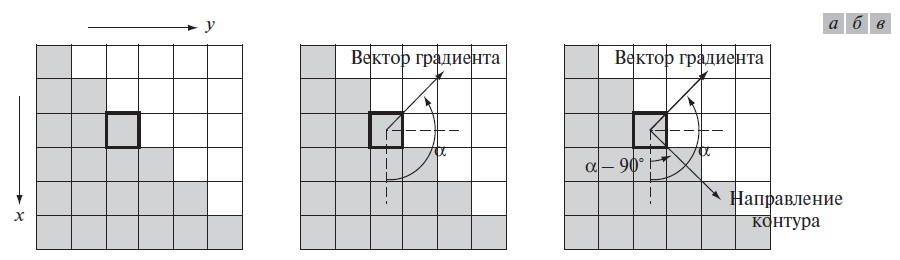
\includegraphics[width=0.7\linewidth]{grad.jpg}
	
	\caption{Применение градиента для нахождения границ контуров на изображении}
	
	\label{fig:grad}
	
\end{figure}

\newpage

При работе с изображениями функция яркости имеет дискретную природу, поэтому вместо производных первого и второго порядка используются их дискретные аналоги.

Первая производная одномерной функции может быть задана как разность значений соседних элементов:
\begin{gather}\label{first}
	\frac{\partial f}{\partial x}=
	f(x+1) - f(x)
\end{gather}

Аналогично вторая производная определяется как разность соседних значений первой производной:
\begin{gather}\label{second}
	\frac{\partial^2 f}{\partial^2 x}=
	f(x+1) + f(x-1) -2f(x)
\end{gather}

Нетрудно заметить, что по факту эти преобразования задают максимально простые маски фильтрации:
\ref{grad_mask}-$a$ для первой производной вертикальной компоненты и \ref{grad_mask}-$b$~--- для второй.
\begin{gather}\label{grad_mask}
	\begin{bmatrix} w(x,y)=-1 \\ w(x+1,y)=1 \end{bmatrix}
	~~~~~~~~~~~~~~~~~~~~
	\begin{bmatrix} 
	w(x-1,y)=1 \\ w(x,y)=-2 \\ w(x+1,y)=1 \\
	\end{bmatrix}\\
a~~~~~~~~~~~~~~~~~~~~~~~~~~~~~~~~~~~~~~~~~~~~b\notag
\end{gather}

Однако, способ дискретно приблизить производную, описанный выше не единственный. Так, можно, например, использовать маски размером $3\times3$. Далее описаны другие вариации градиентных операторов.

\subsubsection{Оператор Робертса}

Обозначим область изображения размером $3\times 3$ и значения яркостей к жадой из ее точек в соответствии с рис.~\ref{fig:grad_mask_3}

\begin{figure}[h]
	
	\centering
	
	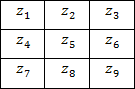
\includegraphics[width=0.2\linewidth]{grad_mask_3.jpg}
	
	\caption{Яркости в области $3\times3$ на изображении}
	
	\label{fig:grad_mask_3}
	
\end{figure}

Один из возможных способов нахождения первых частных производных в точке~$z_5$ состоит в применении перекрестного оператора Робертса:
\begin{gather}\label{grad_mask_3}
	g_x = \frac{\partial f}{\partial x} = (z_9-z_5)\\
	g_y = \frac{\partial f}{\partial y} = (z_8-z_6)
\end{gather}

Такое преобразование задает маски фильтрации на рис.~\ref{fig:grad_mask_rob} соотвественно.

\begin{figure}[h]
	
	\centering
	
	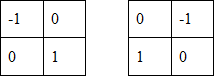
\includegraphics[width=0.25\linewidth]{grad_mask_rob.jpg}
	
	\caption{Маски оператора Робертса}
	
	\label{fig:grad_mask_rob}
	
\end{figure}

Основным преимуществом данного градиентного оператора является высокая скрость обработки изображения, но зачастую устойчивость оставляет желать лучшего. 

\subsubsection{Оператор Превитта}

Используем обозначения рис.~\ref{fig:grad_mask_3}. Тогда оператор Превитта может быть задан выражениями:
\begin{gather}\label{grad_mask_prev}
	g_x = \frac{\partial f}{\partial x} = (z_7+z_8+z_9)-(z_1+z_2+z_3)\\
	g_y = \frac{\partial f}{\partial y} = (z_3+z_6+z_9)-(z_1+z_4+z_7)
\end{gather}

Маска этого градиентного оператора имеет вид, изображенный на рис.~\ref{fig:grad_mask_prev}.

\begin{figure}[h]
	
	\centering
	
	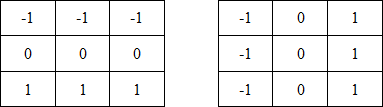
\includegraphics[width=0.4\linewidth]{grad_mask_prev.jpg}
	
	\caption{Маски оператора Превитта}
	
	\label{fig:grad_mask_prev}
	
\end{figure}

\subsubsection{Оператор Собеля}

Небольшое видоизменение формул ~\ref{grad_mask_prev} в виде использования весового коэффициента~$2$ для средних элементов, позволяет уменьшить эффект сглаживания для функции градиента:
\begin{gather}\label{grad_mask_sob}
	g_x = \frac{\partial f}{\partial x} = (z_7+2z_8+z_9)-(z_1+2z_2+z_3)\\
	g_y = \frac{\partial f}{\partial y} = (z_3+2z_6+z_9)-(z_1+2z_4+z_7)
\end{gather}

\newpage

Маски, используемые оператором Собеля, отображены на рис.~\ref{fig:grad_mask_sob}.

\begin{figure}[h]
	
	\centering
	
	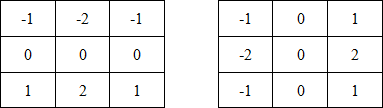
\includegraphics[width=0.4\linewidth]{grad_mask_sob.jpg}
	
	\caption{Маски оператора Собеля}
	
	\label{fig:grad_mask_sob}
	
\end{figure}

Стоит отметить, что у каждой из градиентных масок, описанных выше, сумма весовых коэффициентов равна нулю, то есть эти операторы будут давать нулевой отклик на областях постоянной яркости, как и следовало ожидать от дифференциального оператора.

\subsubsection{Преобразование Хафа}

Рассмотренные выше методы применимы, когда имеется дополнительная информация о местоположении исследуемых объектов на изображении. Зачастую таких данных нет и приходится исходить из заранее заданных глобальных свойств. Ниже изложен метод, основанный на выянении того, лежат ли множества пикселей на кривой заранее заданной формы.
Будем считать, что контур искомой кривой изначально имеет форму прямой, и воспользуемся преобразованием Хафа для ее поиска.
Рассмотрим точку~$(x_i, y_i)$ исходного изображения и общее уравнение прямой на плоскости:$y = ax+b$. Через точку~$(x_i, y_i)$ проходит бесконечное множество прямых, удовлетворяющих уравнению: $y_i = ax_i+b$. Перепишем это уравнение в виде:$b = x_i a - y_i$ и перейдем в координатную плоскость $ab$, называемую пространством параметров. Очевидно, что в нем для заданной пары~$(x_i, y_i)$ существует уравнение единственной прямой. Более того для каждой пары $(x_i, y_i)$,$(x_j, y_j)$ точек в исходном пространстве, в пространстве параметров существует единственная точка $(a', b')$, находящаяся на пересечении соотвествующих для точек прямых пространства параметров и задающая прямую, на которой лежат эти точки в исходном пространстве(рис.~\ref{fig:param_haf}).

\begin{figure}[h]
	
	\centering
	
	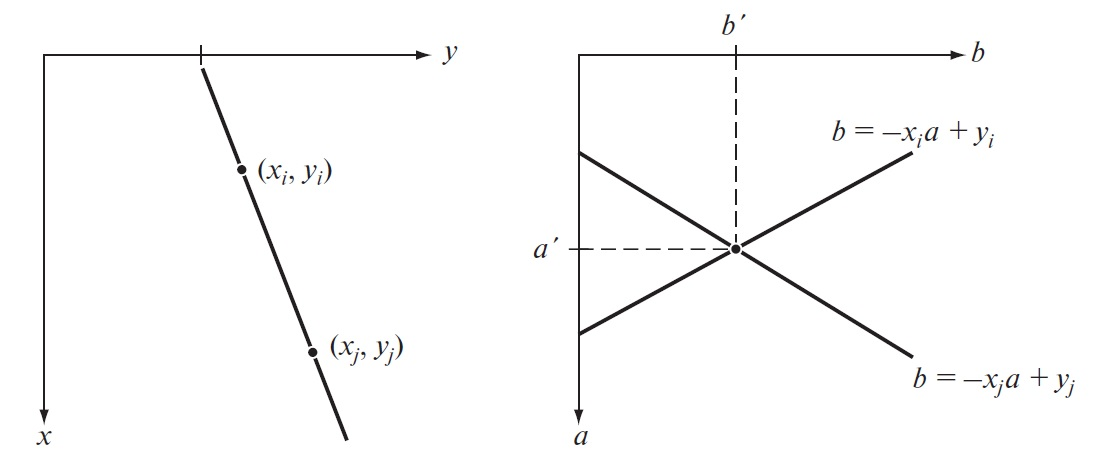
\includegraphics[width=0.6\linewidth]{param_haf.jpg}
	
	\caption{Исходная плоскость($xy$), Пространство параметров($ab$)}
	
	\label{fig:param_haf}
	
\end{figure}

Проблема использования такого перехода проявляется при попытке отобразить прямую близкую к вертикальной, так как ее угловой коэффициент $a$ стремится к бесконечности. Поэтому, чтобы обойти данную трудность прямую представляют с помощью нормали:
\begin{gather}\label{norm}
	x\cos{\Theta} + y\sin{\Theta} = \rho
\end{gather}

Геометрическую интерпретацию параметров~$\rho$~и~$\Theta$ можно увидеть на рис.~\ref{fig:norm}-а. Каждая синусоида на рис.~\ref{fig:norm}-б представляет семейство прямых, проходящих через конкретную точку $(x_k, y_k)$ на исходной плоскости $xy$. Точка перечения $(\rho'\Theta')$ на этом рисунке соответствует прямой, проходящей через точки $(x_i, y_i)$ и $x_j, y_j$ на рис.~\ref{fig:norm}-а.

\begin{figure}[h]
	
	\centering
	
	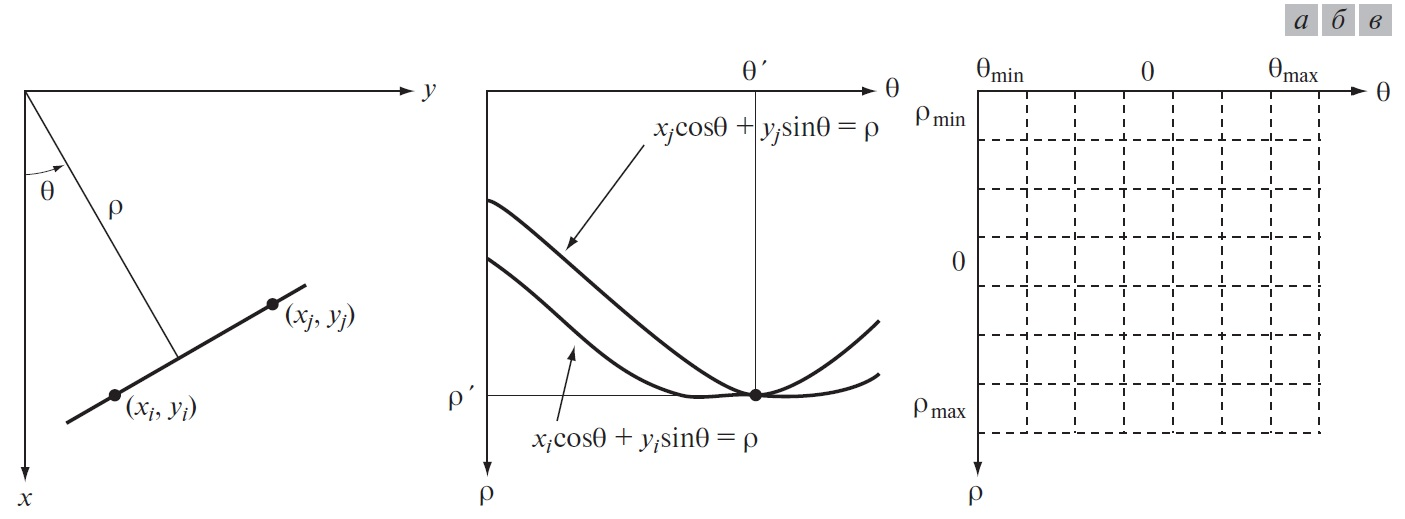
\includegraphics[width=0.8\linewidth]{norm.jpg}
	
	\caption{(а)~Представление прямой на исходной плоскости с помощью параметров нормали $(\rho, \Theta)$. 
	(б)~Синусоиды на плоскости $\rho \Theta$.
	(в)~Разбиение плоскости $\rho \Theta$ на ячейки накопления}
	
	\label{fig:norm}
	
\end{figure}

Осуществив преобразование Хафа, далее предлагается разбить пространство параметров $\rho \Theta$ на так называемые ячейки накопления, как показано на рис.~\ref{fig:norm}-в. Затем для каждой точки $(x_k, y_k)$ исходной плоскости перебираем возможные значения для параметра $\Theta$ и находим соотвествующее ему значение $\rho = x_k\cos{\Theta}+y_k\sin{\Theta}$. Если выбор значения $\Theta_p$ приводит к решению $\rho_q$, то увеличиваем значение ячейки $A(p,q)$ на 1. После выполнения этого алгоритма значение $A(p,q)=Q$ означает, что на исходной плоскости находится $Q$ точек лежащих на прямой $\rho_p = x_k\cos{\Theta_q}+y_k\sin{\Theta_q}$.
Отсюда и находят прямые контура. Аналогичным образом можно применять преобразование Хафа к любой функции вида $g(v,c) = 0$, где $v$~--- это вектор координат, а $c$~--- вектор коэффициентов.

Так любое коническое сечение, в частности парабола, может быть задано уравнением в полярных координатах:
\begin{gather}\label{conic}
	\rho = \frac{de}{1\pm e\cos{\Theta}}~~~\text{или}
	\\
	\rho = \frac{de}{1\pm e\sin{\Theta}},~~~~~~~
\end{gather}
где $e$~--- эксцентриситет и $d$~--- кратчайшее расстояние между фокусом и директрисой. Для конических сечений эксцентриситет имеет разные значения в зависимости от формы кривой. Так для элипса он лежит в диапазоне: $0<e<1$, для гиперболы~--- $e>1$, а для параболы $e = 1$, ее далее и рассмотрим.

Парабола может быть определена как геометрическое множество точек, равноудаленных от неподвижной точки, называемой фокусом и прямой, называемой директрисой(рис.~\ref{fig:hough_parab}). Эта парабола, описывается уравнением:
\begin{gather}\label{parab_equ}
	(y-y_0)^2 = 4a(x-x_0)
\end{gather}

\begin{figure}[h]
	
	\centering
	
	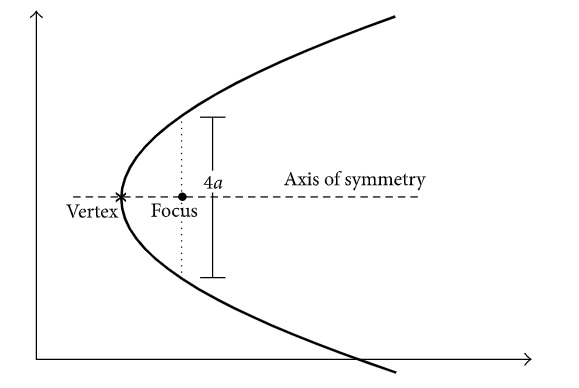
\includegraphics[width=0.7\linewidth]{hough_parab.jpg}
	
	\caption{Парабола}
	
	\label{fig:hough_parab}
	
\end{figure}
Дифференциальное уравнение относительно $x$ может быть получено как:
\begin{gather}\label{parab_diff}
	\frac{\text{d}y}{\text{d}x}=\sqrt{\frac{a}{x-x_0}} = \tan{\lambda}
\end{gather}
Это уранение касательной параболы. В работе [11] было выведено соотношение между углом наклона параболы и углом $\Theta$:
\begin{gather}\label{angl}
	\Theta = 2\lambda
\end{gather}
 
Из геометрических соображений получаем фокусную точку параболы
\subsubsection{Интегро-дифференциальный оператор (IDO)}

Оператор, предложенный в \cite{Daugman2, Daugman4, Daugman, Daugman3}, используется в первую очередь для детектирования объектов круглой формы: в оригинале зрачка и радужки. Но также его автором было предложено детектировать верхние и нижние веки путем настройки поиска контура с кругового на дугообразный.

Интегро-дифференциальный оператор определяестя как:
\begin{gather}\label{norm}
	\max_{r, x_0, y_0}{\left| G_\sigma(r)*\left(\frac{\delta}{\delta r}\right)\int_{r, x_0, y_0}{\frac{I(x,y)}{2\pi r}ds}\right|}
\end{gather}

При непрерывном применении оператора на изображении мы максимизируем исследуемый функционал по трем параметрам $(x_0, y_0)$~--- координаты центра и радиус $r$. Ожидается, что границы зрачка и радужки будут максимизировать производную интеграла по круговым границам, так как на них значения интерсивности резко меняются. $G_\sigma(r)$~--- сглаживающая функция. Для век алгоритм аналогичный, только форма исследуемых траекторий будет иметь другой вид. Существенная проблема для данного метода~--- излишняя зашумленность изображения, которая может породить внезапные перепады у интегрируемого функционала.


\subsubsection{Оператор Кэнни}

Детектор контуров, предложенный в \cite{Canny}, составляет многоступенчатый алгоритм для обнаружения контуров различной формы и природы. Последовательность действий может быть описана таким образом:

\begin{enumerate}
	\item Применить гауссовский фильтр для сглаживания изображения и удаления шума;
	\item Найти градиенты интенсивности изображения;
	\item Подавить немаксимумы для корректного определения границ;
	\item Применить пороговую фильтрацию для определения потенциальных контуров;
	\item Выделение наиболее весомых контуров.
\end{enumerate}

\textbf{Фильтр Гаусса}

Уравнение, задающее ядро Гауссовского фильтра размера $(2k+1)\times (2k+1)$:
\begin{gather}\label{norm}
	H_{ij}=\frac{1}{2\pi \sigma^2}\exp{\left(\ \frac {-(i-(k+1))^2+(j-(k+1))^2}{2\sigma^2}\right)};~~1\leq i, j \leq(2k+1)
\end{gather}

Очевидно, выбор ядра сглаживания влияет на производительность детектора. Чем больше размер фильтра, тем ниже чувствительность к шуму, но тем больше шансы потерять важную информацию.

\newpage

\subsection{Модели аппроксимации века}

\subsubsection{Эллиптический контур века}

Один из возможных способов приблизить линию века~--- описать ее с помощью эллиптической кривой. Эта модель основана на предположении, что глазное яблоко имеет сферическую форму:
\begin{gather}\label{norm}
	x^2+y^2+z^2= R^2
\end{gather}

Такое предположение приводит к модели, основанной на открытости глаза. Степень открытости~--- угловое положение века относительно центра сферы. Тогда кривую века можно получить как пересечение сферы глазного яблока с плоскостью проходящей через ось $x$ с углом $\varphi$ относительно оси $z$ (рис.~\ref{fig:glaz4}). Уравнение этой плоскости имеет вид:
\begin{gather}\label{el1}
	\tan{\varphi}= \frac{y}{z}
\end{gather}

А кривая пересечения, моделирующая веко, задается эллиптической кривой:
\begin{gather}\label{el2}
	x^2+\frac{y^2}{\sin{\varphi}^2}=R^2
\end{gather}

\begin{figure}[h]
	
	\centering
	
	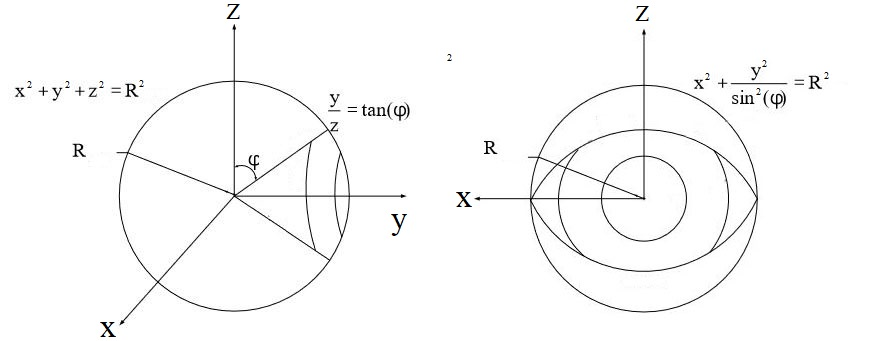
\includegraphics[width=0.8\linewidth]{glaz4.jpg}
	
	\caption{Вид сбоку и спереди эллиптического контура века}
	
	\label{fig:glaz4}
	
\end{figure}


\subsubsection{Параболический контур века}

На практике оказывается, что определять кривую века как пересечение прямой и сферы довольно грубо. Эмпирическим путем было установлено, что форма века глаза человека гораздо лучше аппроксимируется квадратичной параболой(рис.~\ref{fig:glaz5}). Тогда уравнение параметрической кривой, задающее контур века принимает вид:
\begin{gather}\label{par1}
	y = a(x-x_0)^2 + y_0
\end{gather}

\begin{figure}[h]
	
	\centering
	
	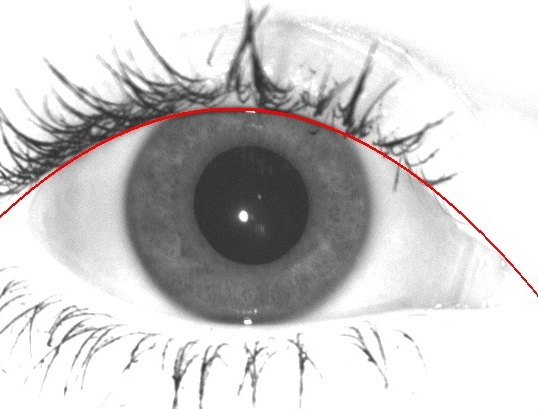
\includegraphics[width=0.6\linewidth]{glaz5.jpg}
	
	\caption{Пример параболического контура века на изображении глаза}
	
	\label{fig:glaz5}
	
\end{figure}

\newpage
\subsection{Методы выделения века на изображении глаза}

В алгоритмах идентификации личности, использующих радужку, чаще всего начинают с опеределения границы радужка-склера \cite{Adam_1, Daugman, Matv} или нормализуют радужку (рис.~\ref{fig:glaz3}) \cite{Min}, а лишь только потом определяют границу века. Это приводит к необходимости выполнять большое количество дополнительных вычислений. Рассмотрим только те методы, в которых для детектирования века необходимо заранее определить не более чем положение зрачка или радужки.

\begin{figure}[h]
	
	\centering
	
	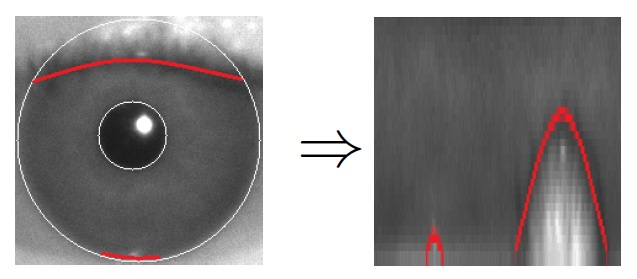
\includegraphics[width=0.8\linewidth]{glaz3.jpg}
	
	\caption{Определение положения века}
	
	\label{fig:glaz3}
	
\end{figure}

Мы можем определить два ключевых этапа в произвольном алгоритме детектирования века на изображении глаза, один из которых ~--- предобработка изображения, а второй~--- локализация века. Как правило, исследователи работают только над одним из этапов, в то время как второй заимствуют из уже ранее написанных работ, предлагая новые комбинации предобработка~-~локализация, которые ранее не были описаны в научной литературе. В данной работе мной проведена оценка существующих методов распознавания и ананлиз методик ранее не упоминавшихся в иcследовательских работах. Предложенный метод сравнивается с наиболее успешными комбинациями, демонстрирующими наиболее точный результат при тестировании.

\textcolor{red}{Планирую расписать этот блок поподробнее, пока просто внес коррективы}

Для нахождения границы века в~\cite{Wildes} предложено использовать в качестве первого шага выделение границ на изображении, а затем для локализации века~--- преобразование~Хафа. 

В \cite{Daugman} используется сглаживание изображения с применением фильтра Гаусса и интегродифференциальный оператор
(IDO) для того, чтобы найти контуры на изображении в том числе нижнее и верхнее веко.

Ещё один метод выделения века предложен в \cite{KKX}, так в работе для предообработки используется одномерный фильтр пиковой формы, хорошо удаляющий шум от ресниц, а для локализации IDO.

Интуитивно понятный метод изложен в \cite{Masek}. Его идея заключается в разделении области радужки и века горизонтальными прямыми, их положение вдоль вертикальной оси определялось значением максимального отклика после осуществления свертки изображения с использованием фильтра Собела. Эта же свертка применяется в \cite{KP} в сочетании с IDO. 

В исследованиях \cite{Adam_2, Adam_1} используется анизотропная диффузия для погашения шумов при предобработке, фильтр Собела для веделения границ и фильтр Хафа для параболлических кривых. 

Для выделения границ в \cite{Yang} предложен ассиметричный оператор Кэнни и для локилизации~--- аппроксимация параболической кривой с помощью МНК. 

В качестве одного из методов определения границ века также можно выделить метод адаптивных контуров, предложенный в работе \cite{Smirn}. Его основная идея~--- задать модель контура последовательностью точек и оптимизировать функционал на этом контуре, таким образом добиваясь его эволюции.

Почти все изложенные выше методы базируются на необходимости наличия дополнительных внешних условий или требований к качеству изображения, поэтому не всегда отличаются хорошей устойчивостью в условиях постоянно изменяющегося окружения. 

%%%%%%%%%%%%%%%%%%%%%%%%%%%%%%%%%%%%%%%%%%%%%%%%%%%%%%

\newpage
\section{Описание модели}

 Предложенный в данной работе метод определения положения век основан на применении вертикального градиента с последующими параболическим преобразованим и преобразованием Радона(рис.~\ref{fig:map})).

\begin{figure}[h]
	
	\centering
	
	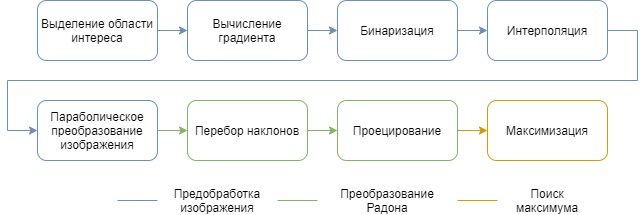
\includegraphics[width=0.8\linewidth]{map.jpg}
	
	\caption{Алгоритм детектирования века на изображении}
	
	\label{fig:map}
	
\end{figure}

В качестве модели кривой, задающей линию века, выбрана параболическая. Как было описано выше, она позволяет довольно четко определить границу века и на практике оказывается выигрышной. Таким образом, основной задачей алгоритма становится определить 3 ключевых параметра: $a, x_0$~и~$y_0$ в~\ref{parab},~--- однозначно определяющих положение века.
\begin{gather}\label{parab}
	y = a(x-x_0)^2 + y_0
\end{gather}

\subsection{Этап предобработки изображения}

В качестве входных данных для алгоритма, помимо самого изображения глаза, используются данные о положении зрачка, а именно координаты его центра и его радиус. Нужны эти данные исключительно для того, чтобы локализировать веко и ускорить обработку изображения. Так, высоту рамки области, в которой мы ищем веко, устанавливаем равной $4\cdot PupR$, где $PupR$~--- это радиус зрачка. А область поиска смещаем на $15\%$ от вертикальной координаты центра зрачка. Также оставляем отсутуп в $5\%$ от горизонтальной координаты центра зрачка слева и справа. Полученный результат локализации изображен на рис.~\ref{fig:glaz6}. Все коэффициенты подобраны опытным путем как наиболее репрезентативные.

\begin{figure}[h]
	
	\centering
	
	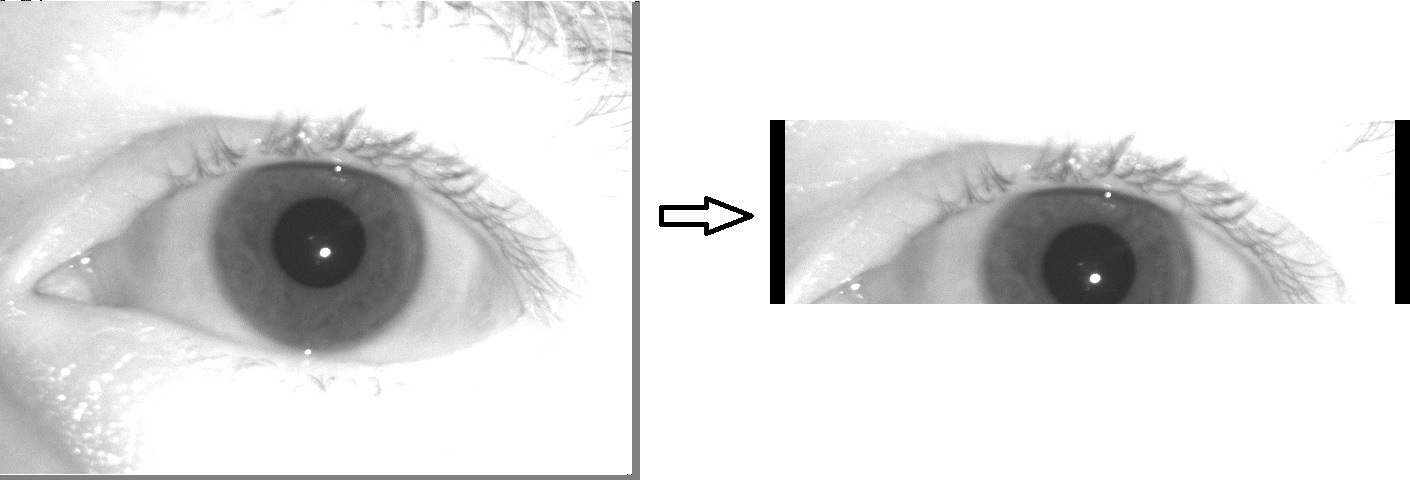
\includegraphics[width=0.8\linewidth]{glaz6.jpg}
	
	\caption{Сужение области поиска}
	
	\label{fig:glaz6}
	
\end{figure}

Заметим, что линия века на фотографии чаще всего сопровождается резким перепадом яркости по вертикали. Соотвественно мы легко можем отследить линию века продифференцировав изображение по вертикальной компоненте(рис.~\ref{fig:glaz7}).

\begin{figure}[h]
	
	\centering
	
	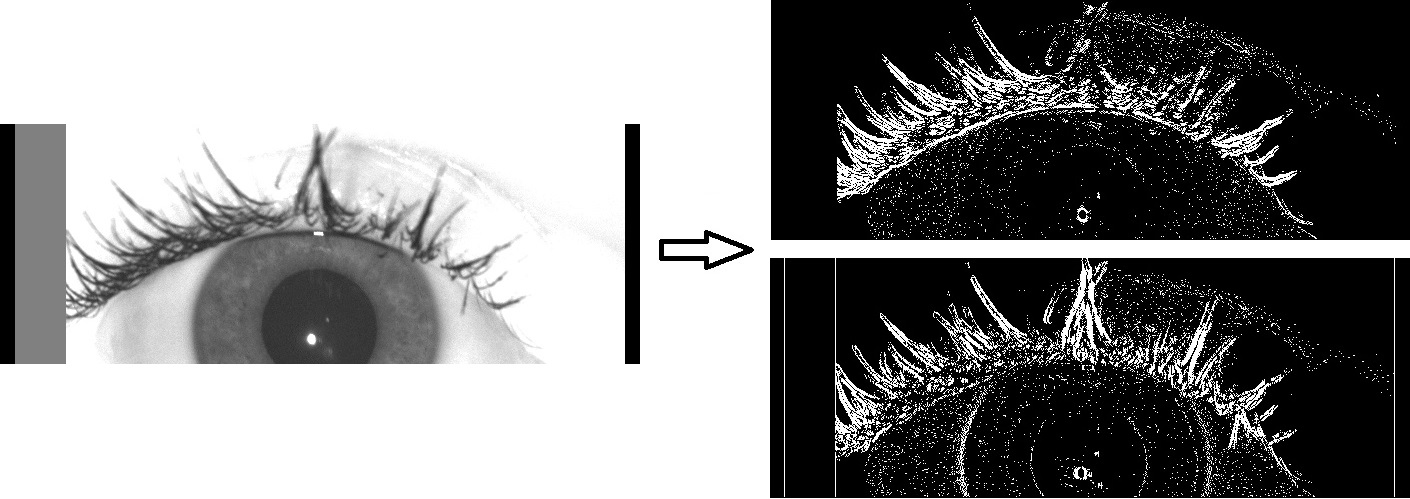
\includegraphics[width=0.8\linewidth]{glaz7.jpg}
	
	\caption{Применение к изображению вертикального и горизонтального градиента с пороговой фильтрацией}
	
	\label{fig:glaz7}
	
\end{figure}

Помимо непосредственного дифференцирования изображения, также применяем пороговую фильтрацию к модулю разницы значений яркостей в соседних пикселях:
\begin{gather}\label{I_diff}
	 I_d(x,y) = \begin{cases}
	 	255, \text{если}~|I(x,y+1) - I(x,y)|> por
	 	\\
	 	0, \text{иначе}
	 \end{cases}
\end{gather}

Величина порогового значения выбрана равной $por=10$ эмпирически.

Заметим, что изображение получилось достаточно зашумленным. Для того, чтобы это исправить, воспользуемся линейной дискретной интерполяцией. Линейное сглаживание по трем точкам~\cite{Inter}~--- это операция усреднения с помощью интерполяционных многочленов, обеспецивающая возможность получения усредненного значения в точке по заданным соседним. Горизонтальное сглаживание задается формулами~\ref{I_glad}, где $X$~--- число пикселей в строке.
\begin{gather}\label{I_glad}
	I_a(x,y) = \begin{cases}
		\frac{5I(0,y)+2I(1,y)-I(2,y)}{6},~\text{если}~x=0
		\\
		\frac{I(x-1,y)+I(x,y)+I(x+1,y)}{3},~\text{если}~1\leq x\leq X-1
		\\
			\frac{5I(X,y)+2I(X-1,y)-I(X-2,y)}{6},~\text{если}~x=X
	\end{cases}
\end{gather}

Однако, так как мы работаем в бинаризованном пространстве, формула выше приобретает вид:
\begin{gather}\label{I_glad_bin}
	I_{a-bin}(x,y) = \begin{cases}
		I_a, \text{если}~I_a = 255
		\\
		0, \text{иначе}
	\end{cases}
\end{gather}

После наложения интерполяционного фильтра изображение приобретает вид рис.~\ref{fig:I_glad}.

\begin{figure}[h]
	
	\centering
	
	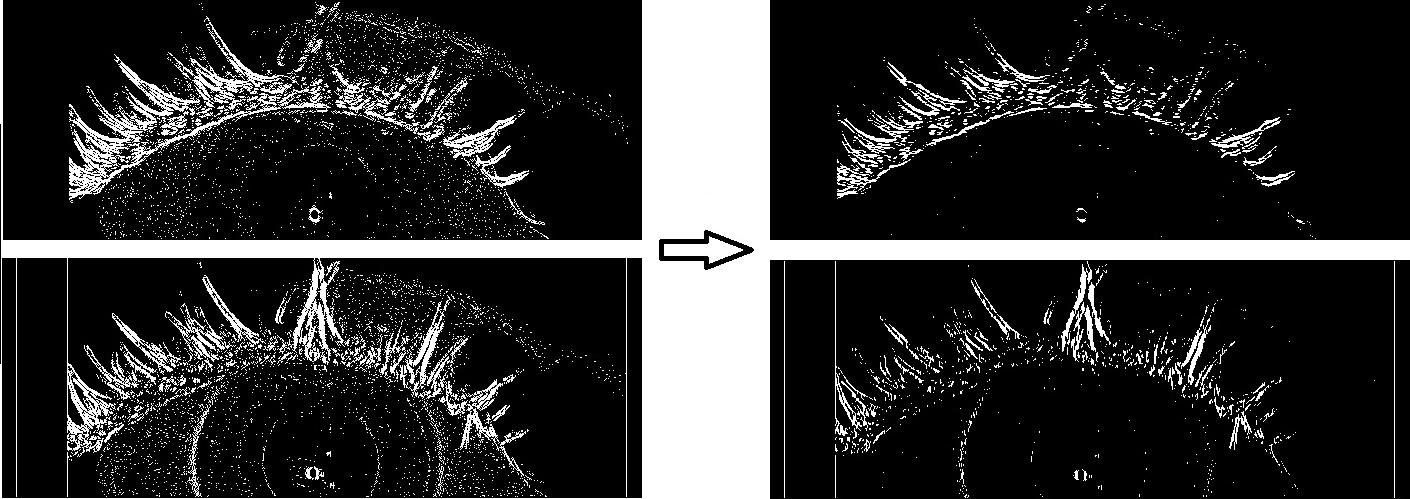
\includegraphics[width=0.8\linewidth]{I_glad.jpg}
	
	\caption{Применение к изображениям вертикального и горизонтального градиента горизонтальной и вертикальной интерполяции соотвественно}
	
	\label{fig:I_glad}
	
\end{figure}

Заметим, что помимо линии века, очень большой вклад в изображение вертикального градиента все еще дают ресницы, однако, на изображении горизонтального градиента веко практически отсутвует, а ресницы все также хорошо видны. Воспользуемся этим моментом для уменьшения шума ресниц рис.~\ref{fig:diff}.
\begin{figure}[h]
	
	\centering
	
	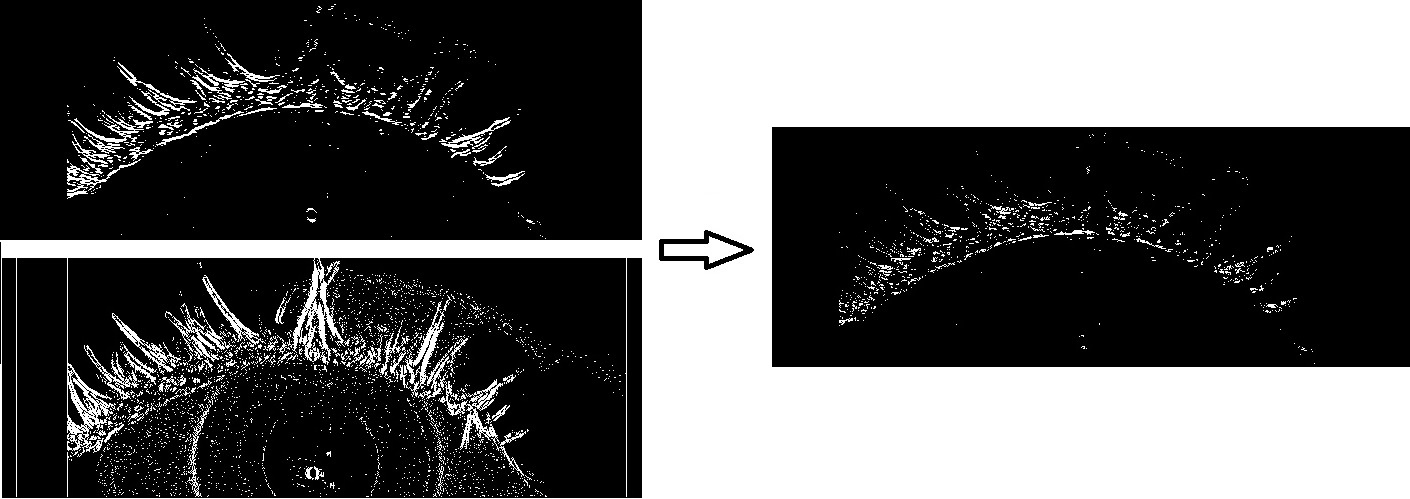
\includegraphics[width=0.8\linewidth]{diff.jpg}
	
	\caption{Уменьшение шума ресниц}
	
	\label{fig:diff}
	
\end{figure}

Последним этапом предобработки изображения является параболическое преобразование. Его можно представить таким образом:
\begin{gather}\label{parab2}
\begin{cases}
		x' = x
		\\
		y' = y - ax^2
	\end{cases},
\end{gather}

где параметр $a$ определяет это преобразование. Заметим, что если в исходном пространстве была задана кривая вида: $y = a(x-x_0) + y_0$, то в пространстве $(y', x')$ она примет вид: $y = -2ax_0\cdot x + (ax_0^2 + y_0) = b\cdot x + c$. Перебирая возможные коэффициенты, мы можем добиться того, чтобы веко приняло форму прямой в конечном пространстве. Пример удачного преобразования на рис.~\ref{fig:parab}.

\begin{figure}[h]
	
	\centering
	
	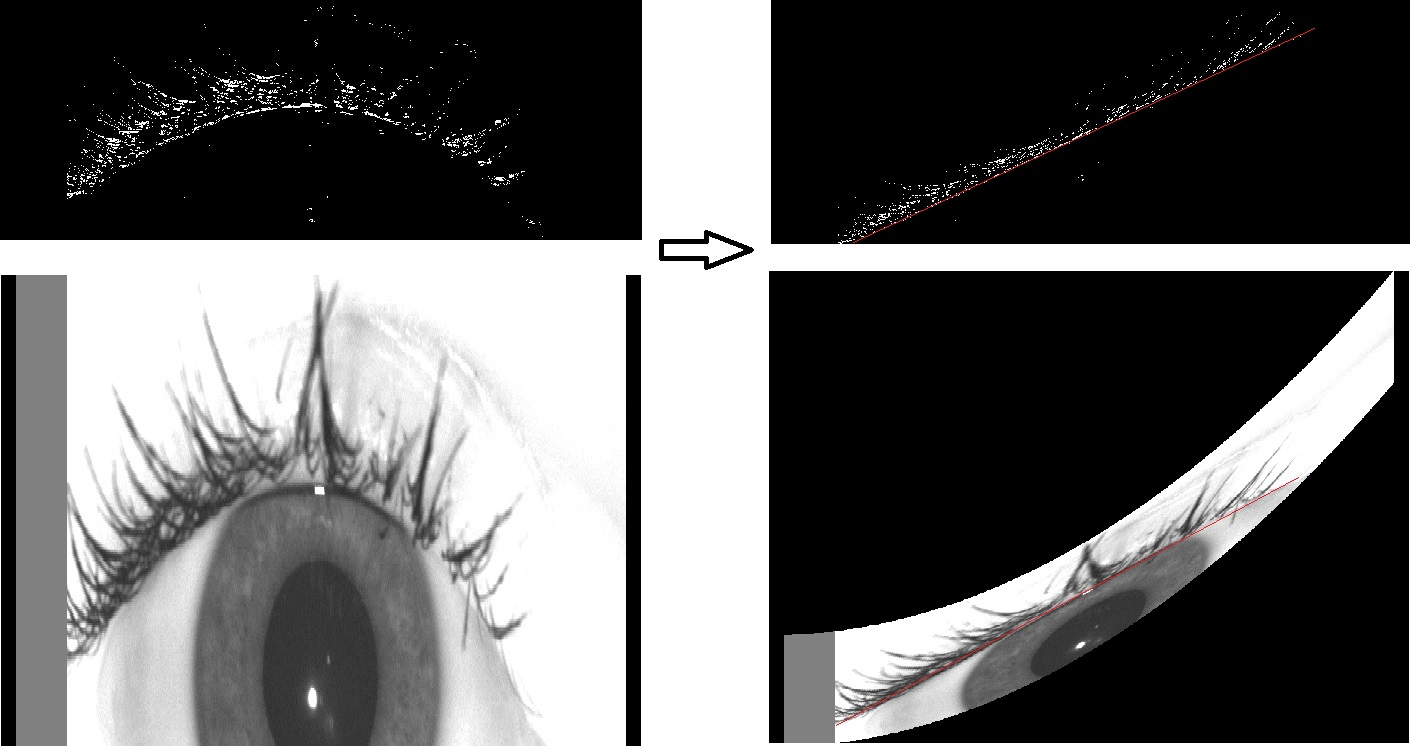
\includegraphics[width=0.8\linewidth]{parab.jpg}
	
	\caption{Параболическое преобразование изображения}
	
	\label{fig:parab}
	
\end{figure}

Теперь необходимо найти прямую и определить её наклон для корректного определения коэффициентов $x_0$ и $y_0$ для века из уравнения выше.
 
\newpage
\subsection{Преобразование Радона}

Рассмотрим простейший случай преобразования Радона, а имеено случай двух переменных. Исходим из предположения, что $f(x,y)$ определена на всей плоскости и достаточно быстро убывает на бесконечности. Последнее условие необходимо для сходимости несобственных интегралов. Тогда преобразованием Радона $f(x,y)$ называется функция~\cite{Radon}:
\begin{gather}\label{radon}
	Rf(s, \alpha) = \int_{-\infty}^{\infty}{f(x(z),y(z))} = \int_{-\infty}^{\infty}{f(s\cos{\alpha}+z\sin{\alpha}, s\sin{\alpha}-z\cos{\alpha})dz}
\end{gather}

Геометрический смысл этого преобразования~--- это интеграл от функции вдоль прямой, перпендекулярной вектору $\vec{n}=(\cos{\alpha}, \sin{\alpha})$ и проходящей на расстоянии $s$ от начала координат вдоль этого вектора (рис.~\ref{fig:Radon_transform}).
\begin{figure}[h]
	
	\centering
	
	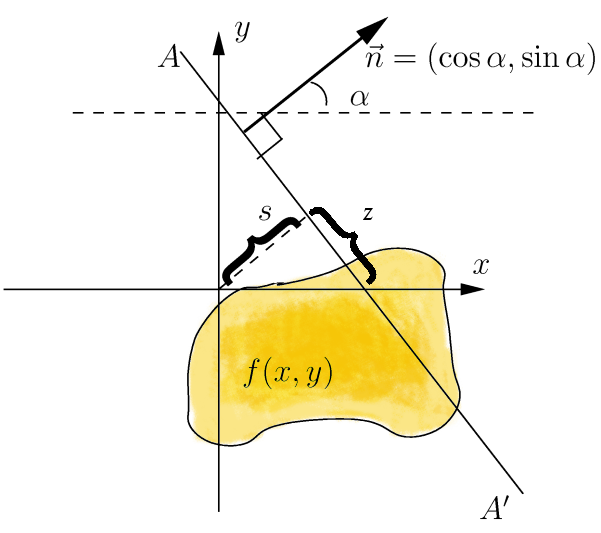
\includegraphics[width=0.5\linewidth]{Radon_transform.jpg}
	
	\caption{Параболическое преобразование изображения}
	
	\label{fig:Radon_transform}
	
\end{figure}

Перейдем к дискретной интерпретации этого метода. Для того, чтобы применить такое преобразование к изображению, можно разделить его на два этапа: выполнить преобразование поворота и просуммировать построчно значения яркостей. Тогда изменение наклона может быть задано формулой:
\begin{gather}\label{nakl}
	\begin{cases}
		x' = x
		\\
		y' = y - bx
	\end{cases},
\end{gather}

Тогда, если прямая изначально имела вид $y=bx+c$, то после преобразования она примет вид $y = c$. Так как шум на изображении все равно присутсвует, далее нужно максимизировать просуммированное значение яркостей вдоль всех строк изображения. Полученный максимум ожидаем в положении последнего искомого коэффициента $c$. Пример преобразования наклона на рис.~\ref{fig:nakl}

\begin{figure}[h]
	
	\centering
	
	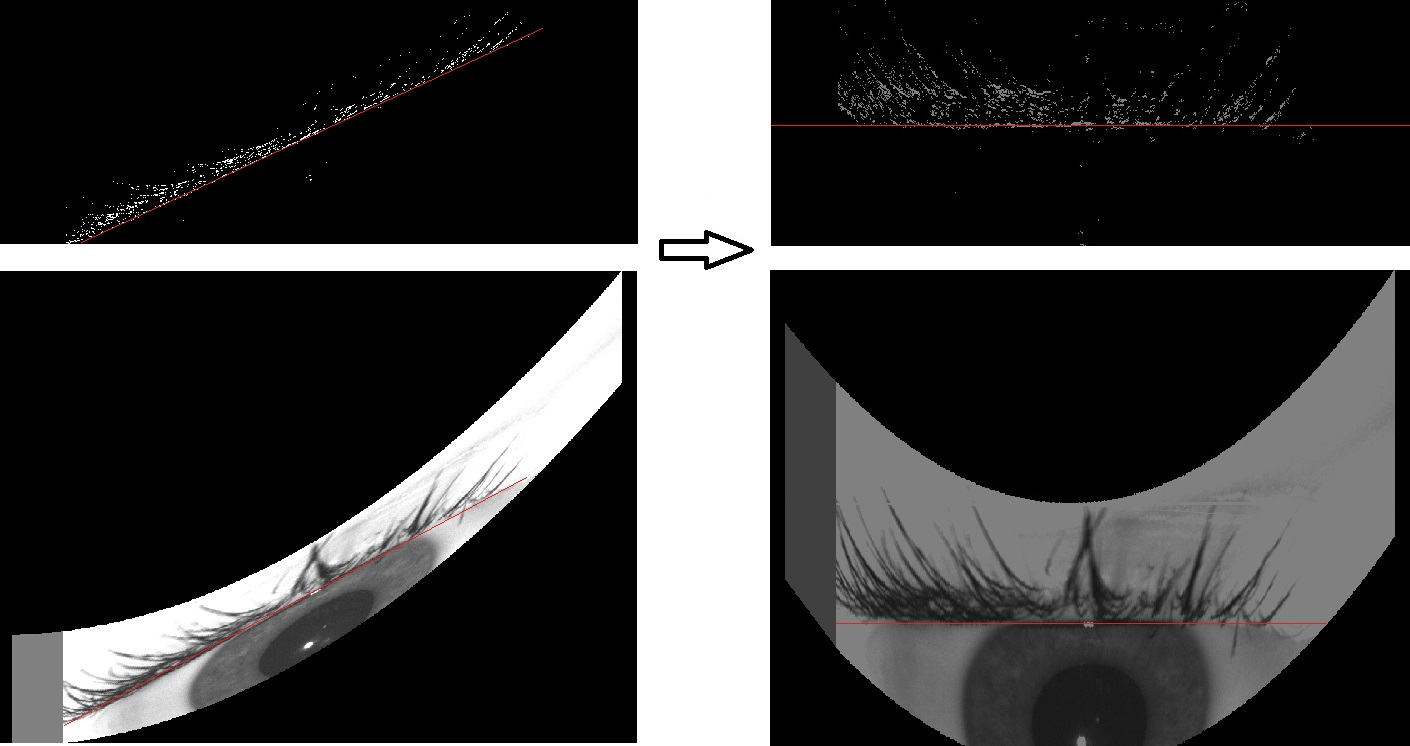
\includegraphics[width=0.8\linewidth]{nakl.jpg}
	
	\caption{Поворот изображения}
	
	\label{fig:nakl}
	
\end{figure}

%%%%%%%%%%%%%%%%%%%%%%%%%%%%%%%%%%%%%%%%%%%%%%%%%%%%%


\newpage
\section{Результаты работы алгоритма}


\begin{figure}[h]
	
	\centering
	
	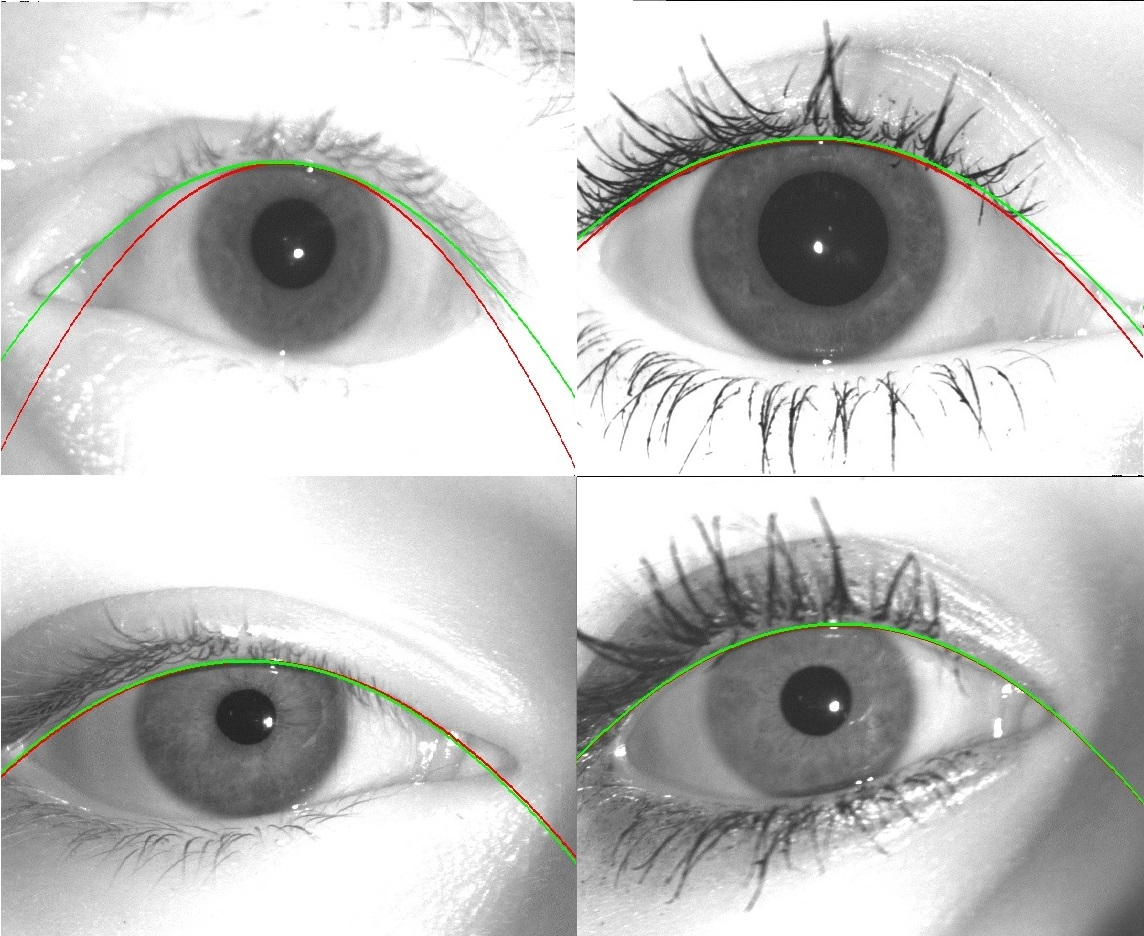
\includegraphics[width=0.6\linewidth]{compare.jpg}
	
	\caption{Сравнение результата с эталоном. Красная линия~--- эталон, зеленая~--- результат алгоритма}
	
	\label{fig:compare}
	
\end{figure}


%%%%%%%%%%%%%%%%%%%%%%%%%%%%%%%%%%%%%%%%%%%%%%%%%%%%%


\newpage
\section{Заключение}


%%%%%%%%%%%%%%%%%%%%%%%%%%%%%%%%%%%%%%%%%%%%%%%%%%%%%


\newpage

\bibliographystyle{plain}
\bibliography{mylib}
\nocite{Yang}

\end{document}